%%%%(c) COPYRIGHT NOTICE%FOLDUP
%%%%(c)
%%%%(c)  This file is a portion of the source for the textbook
%%%%(c)
%%%%(c)    Numerical Methods Course Notes,
%%%%(c)    Copyright 2004-2010 by Steven E. Pav
%%%%(c)
%%%%(c)  See the file COPYING.txt for copying conditions
%%%%(c)
%%%%(c)%UNFOLD

%%throat clearing%FOLDUP
\typeout{-- rootfind.tex}
\typeout{-- N� 2004-2010 Steven E. Pav}
%UNFOLD

%%local commands%FOLDUP
%UNFOLD

\chapter{Finding Roots}\label{chap:rootfind}

%%%%%%%%%%%%%%%%%%%%%%%%%%%%%%%%%%%%%%%%%%%%%%%
\section{Bisection}%FOLDUP

We are now concerned with the problem of finding a zero for the function
$f(x),$ \ie some $c$ such that $f(c) = 0.$

The simplest method is that of bisection.  The following theorem, from calculus
class, insures the success of the method

\begin{bktheorem}[Intermediate Value Theorem]%FOLDUP
If $f(x)$ is continuous on \clinv{a}{b} then for any $y$ such that $y$ is
between $f(a)$ and $f(b)$ there is a $c \in \clinv{a}{b}$ such that $f(c) = y.$
\end{bktheorem}%UNFOLD
\index{Intermediate Value Theorem}

The IVT is best illustrated graphically.  Note that continuity is really a
requirement here--a single point of discontinuity could ruin your whole day, as
the following example illustrates.

\begin{bkexample}%FOLDUP
The function $f(x) = \oneby{x}$ is not continuous at $0$.  Thus if $0 \in
\clinv{a}{b},$ we \emph{cannot} apply the IVT.  In particular, if $0 \in \clinv{a}{b}$
it happens to be the case that for \emph{every} $y$ between $f(a),f(b)$ there
is no $c \in \clinv{a}{b}$ such that $f(c) = y.$
\end{bkexample}%UNFOLD

In particular, the IVT tells us that
if $f(x)$ is continuous and we know $a,b$ such that $f(a),f(b)$ have different
sign, then there is some root in \clinv{a}{b}.  A decent estimate of the root
is $c = \half[a+b].$  We can check whether $f(c) = 0.$  If this does not hold
then one and only one of the two following options holds:
\begin{compactenum}
\item $f(a),f(c)$ have different signs.
\item $f(c),f(b)$ have different signs.
\end{compactenum}
We now choose to recursively apply bisection to either \clinv{a}{c} or
\clinv{c}{b}, respectively, depending on which of these two options hold.

\subsection{Modifications} 
Unfortunately, it is impossible for a computer to test
whether a given black box function is continuous.  Thus malicious or
incompetent users could cause a \naively implemented bisection algorithm to
fail.  There are a number of easily conceivable problems:

\begin{compactenum}
\item The user might give $f,a,b$ such that $f(a),f(b)$ have the same sign.  In
this case the function $f$ might be legitimately continuous, and might have a
root in the interval \clinv{a}{b}.  If, taking $c = \half[a+b],$
$f(a),f(b),f(c)$ all have the same sign, the algorithm would be at an impasse.
We should perform a ``sanity check'' on the input to make sure $f(a),f(b)$ have
different signs.
\item The user might give $f,a,b$ such that $f$ is not continuous on
\clinv{a}{b}, moreover has no root in the interval \clinv{a}{b}.   For a poorly
implemented algorithm, this might lead to an infinite search on smaller and
smaller intervals about some discontinuity of $f$.  In fact, the algorithm
might descend to intervals as small as machine precision, in which case the
midpoint of the interval will, due to rounding, be the same as one of the
endpoints, resulting in an infinite recursion.
\item The user might give $f$ such that $f$ has no root $c$ that is
representable in the computer's memory.  Recall that we think of computers as
storing numbers in the form \tenex{\pm r}{k};  given a finite number of bits to
represent a number, only a finite number of such numbers can be represented.
It may legitimately be the case that none of them is a root to $f$.  In this
case, the behaviour of the algorithm may be like that of the previous case.
A well implemented version of bisection should check the length of its input
interval, and give up if the length is too small, compared to machine
precision.
\end{compactenum}

Another common error occurs in the testing of the signs of $f(a),f(b).$  A
slick programmer might try to implement this test in the pseudocode:
\begin{verbatim}
if (f(a)f(b) > 0) then ...
\end{verbatim}
Note however, that $\abs{f(a)},\abs{f(b)}$ might be very small, and that
$f(a)f(b)$ might be too small to be representable in the computer;   this
calculation would be rounded to zero, and unpredictable behaviour would ensue.
A wiser choice is
\begin{verbatim}
if (sign(f(a)) * sign(f(b)) > 0) then ...
\end{verbatim}
where the function $\operatorname{sign}\Parens{x}$ returns $-1,0,1$ depending
on whether $x$ is negative, zero, or positive, respectively.

The pseudocode bisection algorithm is given as \algref{run_bisection}.
\index{bisection method}

\begin{algorithm}[h]
\caption{Algorithm for finding root by bisection.\label{alg:run_bisection}}
\alginout{a function, two endpoints, a $x$-tolerance, and a $y$-tolerance}{a
$c$ such that $\abs{f(c)}$ is smaller than the $y$-tolerance.}
\algname{run\_bisection}{$f, a, b, \delta, \epsilon$}
\begin{algtab}
	Let $fa \gets \operatorname{sign}\Parens{f(a)}.$\\
	Let $fb \gets \operatorname{sign}\Parens{f(b)}.$\\
	\algif{$fa fb > 0$}
	throw an error.\\
	\algelseif{$fa fb = 0$}
		\algif{$fa = 0$}
			\algreturn $a$\\
		\algelse
			\algreturn $b$\\
		\algend
	\algend
	Let $c \gets \half[a+b]$\\
	\algwhile{$b-a > 2\delta$}
		Let $fc \gets f(c).$\\
		\algif{$\abs{fc} < \epsilon$}
			\algreturn $c$\\
		\algend
	\algif{$\operatorname{sign}\Parens{fa}\operatorname{sign}\Parens{fc} < 0$}
		Let $b \gets c,\, fb \gets fc,\, c \gets \half[a+c].$\\
	\algelse
		Let $a \gets c,\, fa \gets fc,\, c \gets \half[c+b].$\\
	\algend
	\algend
	\algreturn $c$\\
\end{algtab}
\end{algorithm}

\subsection{Convergence}%FOLDUP

We can see that each time $\mathtt{recursive\_bisection}\Parens{f,a,b,\ldots}$
is called that $\abs{b-a}$ is half the length of the interval in the previous
call. Formally call the first interval \clinv{a_0}{b_0}, and the first midpoint
$c_0$.  Let the second interval be \clinv{a_1}{b_1}, etc.  Note that one of
$a_1,b_1$ will be $c_0,$ and the other will be either $a_0$ or $b_0.$  We are
claiming that 
\begin{eqnarray*}
b_n - a_n &=& \half[b_{n-1} - a_{n-1}]\\
	&=& \frac{b_0 - a_0}{2^n}
\end{eqnarray*}

\begin{bktheorem}[Bisection Method Theorem]%FOLDUP
If $f(x)$ is a continuous function on \clinv{a}{b} such that $f(a)f(b) < 0,$
then after $n$ steps, the algorithm $\mathtt{run\_bisection}$ will return $c$
such that $\abs{c-c'} \le \frac{\abs{b-a}}{2^n},$ where $c'$ is some root of
$f$.
\end{bktheorem}%UNFOLD
%UNFOLD
%UNFOLD
%%%%%%%%%%%%%%%%%%%%%%%%%%%%%%%%%%%%%%%%%%%%%%%
\section{Newton's Method}%FOLDUP
\label{sec:newtons}
\depson{sec:taylors}{sec:newtons}

Newton's method is an \emph{iterative} method for root finding.  That is,
starting from some guess at the root, $x_0,$ one iteration of the algorithm
produces a number $x_1,$ which is supposed to be closer to a root; guesses
$x_2,x_3,\ldots,x_n$ follow identically.

Newton's method uses ``linearization'' to find an approximate root.  
Recalling Taylor's Theorem, we know that 
$$f(x+h) \approx f(x) + f'(x) h.$$
This approximation is better when $f''(\cdot)$ is ``well-behaved'' between $x$
and $x+h$. Newton's method attempts to find some $h$ such that
$$0 = f(x+h) = f(x) + f'(x) h.$$
This is easily solved as
$$h = \frac{-f(x)}{f'(x)}.$$

\begin{figure}[htb]%FOLDUP
\begin{center}
\psfrag{x1}{$x_{k}$}
\psfrag{x0}{$x_{k-1}$}
\psfrag{fx1}{$f(x_{k})$}
\psfrag{fx0}{$f(x_{k-1})$}
\includegraphics[width=0.6\columnwidth,angle=270,clip=]{nr.eps}
\end{center}
\caption{One iteration of Newton's method is shown for a quadratic function
$f(x).$  The linearization of $f(x)$ at $x_k$ is shown.  It is clear that
$x_{k+1}$ is a root of the linearization.  It happens to be the case that
$\abs{f(x_{k+1})}$ is smaller than $\abs{f(x_{k})},$ \ie $x_{k+1}$ is a better
guess than $x_k.$}\label{fig:nr}
\end{figure}%UNFOLD

An iteration of Newton's method, then, takes some guess $x_k$ and returns
$x_{k+1}$ defined by
\begin{empheq}[innerbox=\widefbox]{equation}
x_{k+1} = x_k - \frac{f(x_k)}{f'(x_k)}.
\label{eqn:newtonmethod}
\end{empheq}

An iteration of Newton's method is shown in \figref{nr}, along with the
linearization of $f(x)$ at $x_k.$

\subsection{Implementation} Use of Newton's method requires that the function $f(x)$
be differentiable.  Moreover, the derivative of the function must be known.
This may preclude Newton's method from being used when $f(x)$ is a black box.
As is the case for the bisection method, our algorithm cannot explicitly check
for continuity of $f(x).$  Moreover, the success of Newton's method is
dependent on the initial guess $x_0.$  This was also the case with bisection,
but for bisection there was an easy test of the initial interval--\ie test
if $f(a_0)f(b_0) < 0$.

Our algorithm will test for goodness of the estimate by looking at
$\abs{f(x_k)}.$   The algorithm will also test for near-zero derivative.  Note
that if it were the case that $f'(x_k) = 0$ then $h$ would be ill defined.

\index{Newton's Method}
\begin{algorithm}[htb!]%FOLDUP
\caption{Algorithm for finding root by Newton's Method.\label{alg:run_newton}}
\alginout{a function, its derivative, an initial guess, an iteration limit, and a tolerance}{a point for which the function has small value.}
\algname{run\_newton}{$f, f', x0, N, tol$}
\begin{algtab}
	Let $x \gets x0, n \gets 0.$\\
	\algwhile{$n \le N$}
	Let $fx \gets f(x).$\\
	\algif{$\abs{fx} < tol$}
		\algreturn $x.$\\
	\algend
	Let $fpx \gets f'(x).$\\
	\algif{$\abs{fpx} < tol$}
		Warn ``$f'(x)$ is small; giving up.''\\
		\algreturn $x.$\\
	\algend
	Let $x \gets x - fx/fpx.$\\
	Let $n \gets n+1$.\\
	\algend
\end{algtab}
\end{algorithm}%UNFOLD

\subsection{Problems} As mentioned above, convergence is dependent on $f(x),$ and
the initial estimate $x_0.$  A number of conceivable problems might come up.
We illustrate them here.

\begin{bkexample}\label{bkex:xtothej}%FOLDUP
Consider Newton's method applied to the function $f(x) = x^j$ with $j>1,$ and
with initial estimate $x_0 \ne 0.$
\\Note that $f(x) = 0$ has the single root $x=0.$  Now note that
$$x_{k+1} = x_k - \frac{x_k^j}{j x_k^{j-1}} = \Parens{1 - \oneby{j}} x_k.$$
Since the equation has the single root $x=0,$ we find that $x_{k}$ is
converging to the root.  However, it is converging at a rate slower than we
expect from Newton's method: at each step we have a constant decrease of $1 -
\oneBy{j},$ which is a larger number (and thus worse decrease) when $j$ is
larger.
\end{bkexample}%UNFOLD
\begin{bkexample}\label{bkex:runaway}%FOLDUP
Consider Newton's method applied to the function $f(x) = \frac{\ln x}{x},$ with
initial estimate $x_0 = 3.$
\\Note that $f(x)$ is continuous on \reals{+}.  It has a single root at $x=1.$
Our initial guess is not too far from this root.  However, consider the
derivative:
\begin{eqnarray*}
f'(x) &=& \frac{x \oneby{x} - \ln x}{x^2} = \frac{1 - \ln x}{x^2}
\end{eqnarray*}
If $x > \exp{1},$ then $1 - \ln x < 0,$ and so $f'(x) < 0.$  However, for $x >
1,$ we know $f(x) > 0.$  Thus taking
$$x_{k+1} = x_k - \frac{f(x_k)}{f'(x_k)} > x_k.$$
The estimates will ``run away'' from the root $x=1.$
\end{bkexample}%UNFOLD
\begin{bkexample}\label{bkex:newtpong}%FOLDUP
Consider Newton's method applied to the function $f(x) = \sin\Parens{x}$ for
the initial estimate $x_0 \ne 0,$ where $x_0$ has the odious property $2 x_0 =
\tan{x_0}.$
\\You should verify that there are an infinite number of such $x_0$.  Consider
the identity of $x_1:$
$$x_1 = x_0 - \frac{f(x_0)}{f'(x_0)} = x_0 - \frac{\sin(x_0)}{\cos(x_0)} 
= x_0 - \tan{x_0} = x_0 - 2 x_0 = - x_0.$$
Now consider $x_2:$
$$x_2 = x_1 - \frac{f(x_1)}{f'(x_1)} = - x_0 - \frac{\sin(- x_0)}{\cos(- x_0)} 
 - x_0 + \frac{\sin(x_0)}{\cos(x_0)} 
= - x_0 + \tan{x_0} = - x_0 + 2 x_0 = x_0.$$
Thus Newton's method ``cycles'' between the two values $x_0,-x_0$.
\end{bkexample}%UNFOLD

Of course, Newton's method may find some iterate $x_k$ for which $f'(x_k) = 0,$
in which case, there is no well-defined $x_{k+1}.$

\subsection{Convergence} %FOLDUP
%cut the proof%FOLDUP
%Assume that $f(x)$ has two continuous derivatives, and that
%it has some simple root $r,$ \ie we assume that $f(r) = 0 \ne f'(r).$
%Let $e_k = r - x_k,$ the distance from $x_k$ to the root $r.$  Then
%\begin{eqnarray*}
%e_{k+1} &=& r - x_{k+1} = r - x_k + x_k - x_{k+1},\\
%&=& e_k + x_k - x_{k+1},\\
%&=& e_k + \frac{f(x_k)}{f'(x_k)},\\
%&=& \frac{f'(x_k)e_k + f(x_k)}{f'(x_k)}.
%\end{eqnarray*}
%
%Now recall Taylor's theorem, expanding about $x_k$:
%\begin{eqnarray*}
%0 = f(r) = f(r - x_k + x_k) = f(x_k + e_k) &=& f(x_k) + f'(x_k)
%e_k + \half[f''(\xi_k)]e_k^2,
%\end{eqnarray*}
%where $\xi_k$ is between $x_k$ and $r = x_k+e_k.$ 
%
%Then
%\begin{eqnarray*}
%e_{k+1} &=& \frac{-f''(\xi_k)e_k^2}{2f'(x_k)}.
%\end{eqnarray*}
%
%
%Now consider the oddball function
%$$
%c(\delta) = \half \frac{\max_{\abs{x-r} \le \delta} \abs{f''(x)}}
%{\min_{\abs{x-r} \le \delta} \abs{f'(x)}},
%$$
%for $\delta > 0.$  Note that by definition $c(\delta)$ is increasing in
%$\delta,$ and that 
%$$\lim_{\delta \to 0^{+}} c(\delta) = \half \frac{f''(r)}{f'(r)} = z.$$
%By the assumption that $r$ is a simple root, $z$ is finite.  Then there is some
%$D$ such that $\delta \le D \implies \delta c(\delta) \le \half.$
%
%Now if $\abs{r - x_k} = \abs{e_k} < D,$ then $\xi_k,$ which is between $r$ and
%$x_k$ is also near $r$: $\abs{r - \xi_k} < D.$  In this case
%\begin{eqnarray*}
%\abs{e_{k+1}} &=& \abs{\frac{-f''(\xi_k)}{2f'(x_k)}}\abs{e_k^2},\\
% &=& \abs{\frac{-f''(\xi_k)}{2f'(x_k)}}\abs{e_k} \abs{e_k},\\
% &\le& C(D) D \abs{e_k} \le \half \abs{e_k} < D.
%\end{eqnarray*}
%Thus if $\abs{e_k} < D,$ then $\abs{e_{k+1}} < D,$ and so $\abs{e_n} < D$ for
%$n > k.$  Moreover
%\begin{eqnarray*}
%\abs{e_{k+1}} &=& \abs{\frac{-f''(\xi_k)}{2f'(x_k)}}\abs{e_k^2},\\
% &\le& c(D) \abs{e_k^2}.
%\end{eqnarray*}
%UNFOLD
When Newton's Method converges, it actually displays \emph{quadratic
convergence}. That is, if $e_k = x_k -r,$ where $r$ is the root that the $x_k$
are converging to, that $\abs{e_{k+1}} \le C \abs{e_k}^2.$  
If, for example, it were the case that $C = 1,$ then we
would double the accuracy of our root estimate with each iterate.  That is, if
$e_0$ were $0.001,$ we would expect $e_1$ to be on the order of $0.000001$.
The following theorem formalizes our claim:

\begin{bktheorem}[Newton's Method Convergence]%FOLDUP
If $f(x)$ has two continuous derivatives, and $r$ is a simple root of $f(x),$
then there is some $D$ such that if $\abs{x_0 - r} < D,$ Newton's method will
converge quadratically to $r.$
\end{bktheorem}%UNFOLD

The proof is based on arguments from real analysis, and is omitted;  see Cheney
\& Kincaid for the proof \cite{KdCw1999}.  Take note of the following, though:

\begin{compactenum}
\item The proof requires that $r$ be a simple root, that is that $f'(r) \ne 0.$  
When this does not hold we may get only linear convergence, as in
\bkexref{xtothej}.
\item The key to the proof is using Taylor's theorem, and the definition of
Newton's method to show that
\begin{eqnarray*}
e_{k+1} &=& \frac{-f''(\xi_k)e_k^2}{2f'(x_k)},
\end{eqnarray*}
where $\xi_k$ is between $x_k$ and $r = x_k+e_k.$ 

The proof then proceeds by showing that there is some region about $r$ such
that 
	\begin{compactenum}
	\item in this region $\abs{f''(x)}$ is not too large and $\abs{f'(x)}$ is not
	too small, and
	\item if $x_k$ is in the region, then $x_{k+1}$ is in the region.
	\end{compactenum}
In particular the region is chosen to be so small that if $x_k$ is in the
region, then the factor $e_k^2$ will outweigh the factor
$\abs{f''(\xi_k)}/2\abs{f'(x_k)}.$  You can roughly think of this region as an
``attractor'' region for the root.  
\item The theorem never guarantees that some $x_k$ will fall into the
``attractor'' region of a root $r$ of the function, as in 
\bkexref{runaway} and \bkexref{newtpong}.
The theorem that follows gives sufficient conditions for convergence to a
particular root.
\end{compactenum}
 
\begin{bktheorem}[Newton's Method Convergence II \cite{CsddBc1980}]%FOLDUP
If $f(x)$ has two continuous derivatives on \ccinv{a}{b}, and
\begin{compactenum}
\item $f(a)f(b) < 0,$
\item $f'(x) \ne 0$ on \ccinv{a}{b},
\item $f''(x)$ does not change sign on \ccinv{a}{b},
\item Both $\abs{f(a)} \le (b-a)\abs{f'(a)}$ and 
$\abs{f(b)} \le (b-a)\abs{f'(b)}$ hold,
\end{compactenum}
then Newton's method converges to the unique root of $f(x) = 0$ for any choice
of $x_0 \in \ccinv{a}{b}.$
\end{bktheorem}%UNFOLD

%UNFOLD
\subsection{Using Newton's Method} %FOLDUP

Newton's Method can be used to program more complex functions using only simple
functions. Suppose you had a computer which could perform addition,
subtraction, multiplication, division, and storing and retrieving numbers, and
it was your task to write a subroutine to compute some complex function
$g(\cdot).$  One way of solving this problem is to have your subroutine use
Newton's Method to solve some equation equivalent to $g(z) - x = 0$, where $z$
is the input to the subroutine.  Note that it is assumed the subroutine cannot
evaluate $g(z)$ directly, so this equation needs to be modified to satisfy the
computer's constraints.  

Quite often when dealing with problems of this type, students make the mistake
of using Newton's Method to try to solve a linear equation.  This should be an
indication that a mistake was made, since Newton's Method can solve a linear
equation in a single step:

\begin{bkexample}%FOLDUP
Consider Newton's method applied to the function $f(x) = ax + b.$
The iteration is given as 
$$x_{k+1} \gets x_k - \frac{a x_k + b}{a}.$$
This can be rewritten simply as $x_{k+1} \gets - b/a.$
\end{bkexample}%UNFOLD

The following example problems should illustrate this process of
``bootstrapping'' via Newton's Method.

\begin{bkexprob}\label{bkexp:fakeinvs}%FOLDUP
Devise a subroutine using only subtraction and multiplication that can find the
multiplicative inverse of an input number $z,$ \ie can find $\oneBy{z}.$
\begin{bksolution}
We are tempted to use the linear function $f(x) = \oneBy{z} - x.$ But this is a
linear equation for which Newton's Method would reduce to $x_{k+1} \gets
\oneBy{z}.$  Since the subroutine can only use subtraction and multiplication,
this will not work.

Instead apply Newton's Method to $f(x) = z - \oneBy{x}.$  The Newton step is
$$
x_{k+1} \gets x_k - \frac{z - \oneBy{x_k}}{\oneBy{x_k^2}} = x_k - z x_k^2 + x_k
= x_k \Parens{2 - z x_k}.
$$
Note this step uses only multiplication and subtraction.  The subroutine is
given in \algref{fakeinvs}.
\begin{algorithm}[htb!]%FOLDUP
\caption{Algorithm for finding a multiplicative inverse using simple operations.\label{alg:fakeinvs}}
\alginout{a number}{its multiplicative inverse}
\algname{invs}{$z$}
\begin{algtab}
	if $z = 0$ throw an error.\\
	Let $x \gets \sign{z}, n \gets 0.$\\
	\algwhile{$n \le 50$}
	Let $x \gets x \Parens{2 - z x}.$\\
	Let $n \gets n+1$.\\
	\algend
\end{algtab}
\end{algorithm}%UNFOLD
\end{bksolution}
\end{bkexprob}%UNFOLD
\begin{bkexprob}\label{bkexp:fakesqrt}%FOLDUP
Devise a subroutine using only simple operations which computes the square root of an input number $z$.
\begin{bksolution}
The temptation is to find a zero for $f(x) = \sqrt{z} - x.$ 
However, this equation is linear in $x.$
Instead let $f(x) = z - x^2.$  You can easily see that if $x$ is a positive
root of $f(x) = 0,$ then $x = \sqrt{z}.$  
The Newton step becomes
$$x_{k+1} \gets x_k - \frac{z - x_k^2}{-2x_k}.$$
after some simplification this becomes
$$x_{k+1} \gets \half[x_k] + \frac{z}{2x_k}.$$
Note this relies only on addition, multiplication and division.

The final subroutine is given in \algref{fakesqrt}.

\begin{algorithm}[htb!]%FOLDUP
\caption{Algorithm for finding a square root using simple operations.\label{alg:fakesqrt}}
\alginout{a number}{its square root}
\algname{sqrt}{$z$}
\begin{algtab}
	if $z < 0$ throw an error.\\
	Let $x \gets 1, n \gets 0.$\\
	\algwhile{$n \le 50$}
	Let $x \gets \Parens{x + z/x}/2.$\\
	Let $n \gets n+1$.\\
	\algend
\end{algtab}
\end{algorithm}%UNFOLD

\end{bksolution}
\end{bkexprob}%UNFOLD
%UNFOLD
%UNFOLD
%%%%%%%%%%%%%%%%%%%%%%%%%%%%%%%%%%%%%%%%%%%%%%%
\section{Secant Method}%FOLDUP
\label{sec:secant}
\depson{sec:newtons}{sec:secant}

\begin{figure}[htb!]%FOLDUP
\begin{center}
\psfrag{x1}{$x_{k}$}
\psfrag{x0}{$x_{k-1}$}
\psfrag{fx1}{$f(x_{k})$}
\psfrag{fx0}{$f(x_{k-1})$}
\psfrag{x2}{$x_{k+1}$}
\psfrag{fx2}{$f(x_{k+1})$}
\includegraphics[height=0.6\columnwidth,angle=270,clip=]{sm.eps}
\end{center}
\caption{One iteration of the Secant method is shown for some quadratic function
$f(x).$  The secant line through $\tuple{x_{k-1},f(x_{k-1})}$ and
$\tuple{x_k,f(x_k)}$ is shown.   It happens to be the case that
$\abs{f(x_{k+1})}$ is smaller than $\abs{f(x_{k})},$ \ie $x_{k+1}$ is a better
guess than $x_k.$}\label{fig:sm}
\end{figure}%UNFOLD
The secant method for root finding is roughly based on Newton's method;
however, it is not assumed that the derivative of the function is known, rather
the derivative is approximated by the value of the function at some of the
iterates, $x_k$.  More specifically, the slope of the \emph{tangent} line at
$\tuple{x_k,f(x_k)},$ which is $f'(x_k)$ is approximated by the slope of the
\emph{secant} line passing through $\tuple{x_{k-1},f(x_{k-1})}$ and
$\tuple{x_k,f(x_k)},$ which is 
$$\frac{f(x_k) - f(x_{k-1})}{x_k - x_{k-1}}$$%

Thus the iterate $x_{k+1}$ is the root of this secant line.  That is, it is a
root to the equation
\[\frac{f(x_k) - f(x_{k-1})}{x_k - x_{k-1}} \Parens{x-x_k} = y - f(x_k).\]
Since the root has a $y$ value of $0,$ we have
\begin{align}
\frac{f(x_k) - f(x_{k-1})}{x_k - x_{k-1}} \Parens{x_{k+1}-x_k} &= -
f(x_k),\nonumber\\
{x_{k+1}-x_k} &= - \Parens{\frac{x_k - x_{k-1}}{f(x_k) - f(x_{k-1})}}
f(x_k),\nonumber\\ 
x_{k+1} &= x_k - \Parens{\frac{x_k - x_{k-1}}{f(x_k) - f(x_{k-1})}}
f(x_k).
\end{align}

You will note this is the recurrence of Newton's method, but with the slope
$f'(x_k)$ substituted by the slope of the secant line.  Note also that the
secant method requires two initial guesses, $x_0,x_1,$ but can be used on a
black box function.  The secant method can suffer from some of the same
problems that Newton's method does, as we will see.

An iteration of the secant method is shown in \figref{sm}, along with the
secant line. 

\begin{bkexample}%FOLDUP
Consider the secant method used on $x^3 + x^2 - x -1,$ with $x_0 = 2,x_1 =
\half.$
\\Note that this function is continuous and has roots $\pm 1.$
We give the iterates here:
$$
\begin{array}{ccl}
k & x_k & f(x_k) \\
0 &    2 &    9 \\
1 &  0.5 & -1.125 \\
2 & 0.666666666666667 & -0.925925925925926 \\
3 & 1.44186046511628 & 2.63467367653163 \\
4 & 0.868254072087394 & -0.459842466254495 \\
5 & 0.953491494113659 & -0.177482458876898 \\
6 & 1.00706900811804 & 0.0284762692197613 \\
7 & 0.999661272951803 & -0.0013544492875992 \\
8 & 0.999997617569723 & \tenex{-9.52969840528617}{-06} \\
9 & 1.0000000008072 & \tenex{3.22880033820638}{-09} \\
10 & 0.999999999999998 & \tenex{-7.43849426498855}{-15} 
\end{array}
$$
\end{bkexample}%UNFOLD

\subsection{Problems} As with Newton's method, convergence is dependent on $f(x),$ and
the initial estimates $x_0,x_1.$  We illustrate a few possible problems:

\begin{bkexample}%FOLDUP
Consider the secant method for the function $f(x) = \frac{\ln x}{x},$ with
$x_0 = 3,x_1 = 4.$
\\As with Newton's method, the iterates diverge towards infinity, looking for a
nonexistant root.  We give some iterates here:
$$
\begin{array}{ccl}
k & x_k & f(x_k) \\
0 &    3 & 0.366204096222703 \\
1 &    4 & 0.346573590279973 \\
2 & 21.6548475770851 & 0.142011128224341 \\
3 & 33.9111765137635 & 0.103911011441661 \\
4 & 67.3380435135758 & 0.0625163004418104 \\
5 & 117.820919458675 & 0.0404780904944712 \\
6 & 210.543986613847 & 0.0254089165873003 \\
7 & 366.889164762149 & 0.0160949419231219 \\
8 & 637.060241341843 & 0.010135406045582 \\
9 & 1096.54125113444 & 0.00638363233543847 \\
10 & 1878.34688714646 & 0.00401318169994875 \\
11 & 3201.94672271613 & 0.0025208146648422 \\
12 & 5437.69020766155 & 0.00158175793894727 \\
13 & 9203.60222260594 & 0.000991714984152597 \\
14 & 15533.1606791089 & 0.000621298692241343 \\
15 & 26149.7196085218 & 0.000388975250950428 \\
16 & 43924.8466075548 & 0.000243375589137882 \\
17 & 73636.673898472 & 0.000152191807070607 
\end{array}
$$
\end{bkexample}%UNFOLD
\begin{bkexample}%FOLDUP
Consider Newton's method applied to the function $f(x) = \oneby{1+x^2}
- \oneby{17},$ with initial estimates $x_0 = -1,x_1 = 1.$
\\You can easily verify that $f(x_0) = f(x_1),$ and thus the secant line is
horizontal.  And thus $x_2$ is not defined.
\end{bkexample}%UNFOLD

\index{secant method}
\begin{algorithm}[htb!]%FOLDUP
\caption{Algorithm for finding root by secant method.\label{alg:run_secant}}
\alginout{a function, initial guesses, an iteration limit, and a tolerance}{a point for which the function has small value.}
\algname{run\_secant}{$f, x0, x1, N, tol$}
\begin{algtab}
	Let $x \gets x1, xp \gets x0, fh \gets f(x1), fp \gets f(x0), n \gets 0.$\\
	\algwhile{$n \le N$}
	\algif{$\abs{fh} < tol$}
		\algreturn $x.$\\
	\algend
	Let $fpx \gets (fh - fp) / (x - xp).$\\
	\algif{$\abs{fpx} < tol$}
		Warn ``secant slope is too small; giving up.''\\
		\algreturn $x.$\\
	\algend
	Let $xp \gets x, fp \gets fh.$\\
	Let $x \gets x - fh/fpx.$\\
	Let $fh \gets f(x).$\\
	Let $n \gets n+1$.\\
	\algend
\end{algtab}
\end{algorithm}%UNFOLD
\subsection{Convergence} %FOLDUP


We consider convergence analysis as in Newton's method.  We
assume that $r$ is a root of $f(x),$ and let $e_n = r - x_n.$  Because the
secant method involves two iterates, we assume that we will find some relation
between $e_{k+1}$ and the previous two errors, $e_k,e_{k-1}.$ 

%%cut proof%FOLDUP
%We start with
%\begin{eqnarray}
%e_{k+1} &=& r - x_{k+1} \nonumber \\
%&=& r - \Bracks{x_k - \frac{x_k - x_{k-1}}{f(x_k) - f(x_{k-1})} f(x_k)} ,\nonumber\\
%&=& \frac{r f(x_k)  - r f(x_{k-1})}{f(x_k) - f(x_{k-1})} -
%	\frac{f(x_k) x_{k-1} - f(x_{k-1})x_k}{f(x_k) - f(x_{k-1})} ,\nonumber \\
%&=& \frac{f(x_k) e_{k-1} - f(x_{k-1})e_k}{f(x_k) - f(x_{k-1})} ,\nonumber\\
%&=& \frac{f(x_k)/e_k - f(x_{k-1})/e_{k-1}}{f(x_k) - f(x_{k-1})} e_k e_{k-1}
%,\nonumber\\
%&=& \Bracks{\frac{x_k - x_{k-1}}{f(x_k) - f(x_{k-1})}} \Bracks{\frac{f(x_k)/e_k -
%f(x_{k-1})/e_{k-1}}{x_k - x_{k-1}}} e_k e_{k-1} .\label{eqn:wherestop}
%\end{eqnarray}
%
%Now recall Taylor's theorem, expanding about $r$:
%\begin{eqnarray*}
%f(x_k) = f(r + x_k - r) = f(r - e_k) &=&
%f(r) + f'(r)(-e_k) + f''(r) \half[e_k^2] - f'''(\xi_k) \frac{e_k^3}{6},\\
%&=& f'(r)(-e_k) + f''(r) \half[e_k^2] - f'''(\xi_k) \frac{e_k^3}{6},\\
%f(x_k)/e_k &=& - f'(r) + f''(r) \half[e_k] - f'''(\xi_k) \frac{e_k^2}{6},\\
%&=& - f'(r) + f''(r) \half[e_k] + \bigo{e_k^2}.
%\end{eqnarray*}
%where $\xi_k$ is between $x_k$ and $r = x_k+e_k.$ 
%
%Line up this equation for $k,k-1,$ then subtract to get
%\begin{eqnarray*}
%f(x_k)/e_k - f(x_{k-1})/e_{k-1} &=& f''(r) \half[e_k - e_{k-1}] + \bigo{e_k^2}
%+ \bigo{e_{k-1}^2}.
%\end{eqnarray*}
%Note that $x_k - x_{k-1} = x_k - r + r - x_{k-1} = e_{k-1} - e_k,$ so
%\begin{eqnarray*}
%f(x_k)/e_k - f(x_{k-1})/e_{k-1} &=& -\half[f''(r)] \Bracks{x_k - x_{k-1}} + \bigo{e_k^2}
%+ \bigo{e_{k-1}^2}.
%\end{eqnarray*}
%
%Returning to \eqnref{wherestop}, we get
%\begin{eqnarray*}
%e_{k+1} &\approx& \Bracks{\frac{x_k - x_{k-1}}{f(x_k) - f(x_{k-1})}}
%\Bracks{-\half[f''(r)]} e_k e_{k-1} .
%\end{eqnarray*}
%By Taylor's theorem, the first term is very near $\oneby{f'(r)},$ so
%\begin{eqnarray*}
%e_{k+1} &\approx& - \frac{f''(r)}{2f'(r)} e_k e_{k-1} = C e_k e_{k-1}.
%\end{eqnarray*}
%%UNFOLD

Indeed, this is the case.  Omitting all the nasty details (see Cheney \&
Kincaid \cite{KdCw1999}), we arrive at the imprecise equation:
\begin{eqnarray*}
e_{k+1} &\approx& - \frac{f''(r)}{2f'(r)} e_k e_{k-1} = C e_k e_{k-1}.
\end{eqnarray*}
Again, the proof relies on finding some ``attractor'' region and using
continuity.

We now postulate that the error terms for the secant method follow some power
law of the following type:
$$
\abs{e_{k+1}} \sim A \abs{e_k}^\alpha.
$$
Recall that this held true for Newton's method, with $\alpha = 2.$
We try to find the $\alpha$ for the secant method.
Note that
$$
\abs{e_k} = A \abs{e_{k-1}}^\alpha,
$$
so
$$
\abs{e_{k-1}} = A^{-\oneby{\alpha}} \abs{e_k}^\oneby{\alpha}.
$$
Then we have
$$
A \abs{e_k}^\alpha = \abs{e_{k+1}} = C \abs{e_k}\abs{e_{k-1}} = C
A^{-\oneby{\alpha}} \abs{e_k}^{1+\oneby{\alpha}},
$$
Since this equation is to hold for all $e_k,$ we must have
$$
\alpha = 1 + \oneby{\alpha}.
$$

This is solved by $\alpha = \half \Parens{1+\sqrt{5}} \approx 1.62$.  Thus we
say that the secant method enjoys \emph{superlinear} convergence;  This is
somewhere between the convergence rates for bisection and Newton's method.
%UNFOLD

%UNFOLD
%%%%%%%%%%%%%%%%%%%%%%%%%%%%%%%%%%%%%%%%%%%%%%%
%\section{Exercises}%FOLDUP
\begin{bkexs}
\item Consider the bisection method applied to find the zero of the function
$f(x) = x^2 - 5x + 3,$ with $a_0 = 0, b_0 = 1.$  What are $a_1, b_1$? What are
$a_2, b_2$ ?

%%%%%%%%%%%%%%%%%%%%%%%%%%%%%%%%
\item Approximate $\sqrt{10}$ by using two steps of Newton's method, with 
an initial estimate of $x_0 = 3.$ (\cf \bkexpref{fakesqrt}) Your answer should
be correct to $5$ decimal places.

%%%%%%%%%%%%%%%%%%%%%%%%%%%%%%%%
\item Consider bisection for finding the root to
$\cos{x} = 0$. 
Let the initial interval $I_0$ be \ccinv{0}{2}.
What is the next interval considered, call it $I_1$?
What is $I_2$? $I_6$?

%%%%%%%%%%%%%%%%%%%%%%%%%%%%%%%%
\item What does the sequence defined by 
$$x_0 = 1,\qquad x_{k+1} = \half{x_k} + \oneby{x_k}$$
converge to?

%%%%%%%%%%%%%%%%%%%%%%%%%%%%%%%%
\item Devise a subroutine using only simple operations that finds, via Newton's
Method, the cubed root of some input number $z.$

%%%%%%%%%%%%%%%%%%%%%%%%%%%%%%%%
\item Use Newton's Method to approximate $\sqrt[3]{9}.$  Start with $x_0 = 2.$
Find $x_2.$

%%%%%%%%%%%%%%%%%%%%%%%%%%%%%%%%
\item Use Newton's Method to devise a sequence
$x_0,x_1,\ldots$ such that $x_k \to \ln 10.$
Is this a reasonable way to write a subroutine that, given $z,$ computes
$\ln{z}$? (\emph{Hint:} such a subroutine would require computation of
$\exp{x_k}.$  Is this possible for rational $x_k$ without using a logarithm?
Is it practical?)

%%%%%%%%%%%%%%%%%%%%%%%%%%%%%%%%
\item Give an example (graphical or analytic)
of a function, $f(x)$ for which Newton's Method:
	\begin{compactenum}
	\item Does not find a root for some choices of $x_0.$
	\item Finds a root for every choice of $x_0.$
	\item Falls into a cycle for some choice of $x_0.$
	\item Converges slowly to the zero of $f(x).$
	\end{compactenum}

%%%%%%%%%%%%%%%%%%%%%%%%%%%%%%%%
\item How will Newton's Method perform for finding the root to $f(x) =
\sqrt{\abs{x}} = 0$?

%%%%%%%%%%%%%%%%%%%%%%%%%%%%%%%%
\item Implement the inverse finder described in \bkexpref{fakeinvs}.
Your m-file should have header line like:
\begin{verbatim}
function c = invs(z)
\end{verbatim}
where \texttt{z} is the number to be inverted.  You may wish to use the builtin
function \texttt{sign}.  As an extra termination condition, you should have the
subroutine return the current iterate if $zx$ is sufficiently close to $1,$ say
within the interval \ooinv{0.9999}{0.0001}.
Can you find some $z$ for which the algorithm performs poorly?

%%%%%%%%%%%%%%%%%%%%%%%%%%%%%%%%
\item Implement the bisection method in \octmat.
Your m-file should have header line like:
\begin{verbatim}
function c = run_bisection(f, a, b, tol)
\end{verbatim}
where \texttt{f} is the name of the function.   Recall that \texttt{feval(f,x)} when
\texttt{f} is a string with the name of some function evaluates that function
at \texttt{x}.  This works for builtin functions and m-files.

	\begin{compactenum}
	\item Run your code on the function $f(x) = \cos x,$ with $a_0 = 0, b_0 = 2.$  
	In this case you can set \texttt{f = "cos"}.
	\item Run your code on the function $f(x) = x^2 - 5x + 3,$ with $a_0 = 0, b_0
	= 1.$  In this case you will have to set \texttt{f} to the name of an m-file
	(without the ``.m'') which will evaluate the given $f(x).$
	\item Run your code on the function $f(x) = x - \cos x,$ with $a_0 = 0, b_0 = 1.$  
	\end{compactenum}

%%%%%%%%%%%%%%%%%%%%%%%%%%%%%%%%
\item Implement Newton's Method.
Your m-file should have header line like:
\begin{verbatim}
function x = run_newton(f, fp, x0, N, tol)
\end{verbatim}
where \texttt{f} is the name of the function, and \texttt{fp} is its
derivative.
Run your code to find zeroes of the following functions:
	\begin{compactenum}
	\item $f(x) = \tan x - x.$
	\item $f(x) = x^2 - (2 + \epsilon) x + 1 + \epsilon,$ for $\epsilon$ small.
	\item $f(x) = x^7 - 7x^6 + 21 x^5 - 35 x^4 + 35 x^3 - 21 x^2 + 7 x - 1.$
	\item $f(x) = \Parens{x - 1}^7.$
	\end{compactenum}

%%%%%%%%%%%%%%%%%%%%%%%%%%%%%%%%
\item Implement the secant method
Your m-file should have header line like:
\begin{verbatim}
function x = run_secant(f, x0, x1, N, tol)
\end{verbatim}
where \texttt{f} is the name of the function.
Run your code to find zeroes of the following functions:
	\begin{compactenum}
	\item $f(x) = \tan x - x.$
	\item $f(x) = x^2 + 1.$ \begin{bknote}This function has no zeroes.\end{bknote}
	\item $f(x) = 2 + \sin x.$ \begin{bknote}This function also has no zeroes.\end{bknote}
	\end{compactenum}
\end{bkexs}
%UNFOLD
%for vim modeline: (do not edit)
% vim:ts=2:sw=2:tw=79:fdm=marker:fmr=FOLDUP,UNFOLD:cms=%%s:tags=tags;:syntax=tex:filetype=tex:ai:si:cin:nu:fo=croqt:cino=p0t0c5(0:
